%
% Angepasste FOM Seminarvorlage
%
\documentclass[12pt,a4paper,listof=totoc,bibliography=totoc]{scrartcl}

\usepackage[english]{babel}			% englische Namen/Umlaute
\usepackage[utf8]{inputenc}	    	% Zeichensatzkodierung
\usepackage{fancyhdr}
\usepackage{graphicx}               % Einbinden von Bildern
\usepackage[hidelinks]{hyperref}	% Klickbare Verweise und \autoref{label}
\usepackage[intoc]{nomencl}
\usepackage{setspace}
\usepackage{parskip}
\usepackage{caption}
\usepackage{float}
\usepackage{geometry}
 \geometry{a4paper, left=40mm, right=20mm, top=40mm, bottom=20mm}
\renewcommand{\familydefault}{\sfdefault}

% Bildueberschrift oben und rechtsbuendig
\captionsetup[figure]{labelfont=bf, textfont=bf}
\captionsetup{justification=raggedright,singlelinecheck=false}

%
%	Hier werden Titel, Bearbeiter und das Datum eingetragen
%
\newcommand\svthema{Multi-Cluster Management für Containerumgebungen}
\newcommand\svperson{Christian Frank (\#473088)}
\newcommand\svdatum{\today}
\newcommand\lvname{Wirtschaftsinformatik: IT-Infrastruktur}
\newcommand\lvtyp{WS 2019}
\newcommand\lvinst{FOM - Hochschule für Oekonomie \& Management}
\newcommand\lvbetr{Dipl.-Wirt.-Inf (FH) Frank R. Becker M.A.}

\hypersetup{ % Thema und Author in die Meta-Daten der PDF
  pdftitle={\svthema}, 
  pdfauthor={Christian Frank},
  pdfsubject={Exploring Rancher to manage multi-cluster Kubernetes environments in Enterprise IT},
  pdfkeywords={Rancher, Kubernetes, Multi-Cluster Management}
}

\begin{document}

% Titel
\title{ \huge\textbf{\svthema} }
\author{ {\svperson} \\ \svdatum }
\date{ \normalsize \centering 
\includegraphics[width=0.3\textwidth]{FOM}\\ {\lvname} \\ {\lvbetr} \\ {\lvinst} \\ {\lvtyp} }

% Seitennummer oben
\pagestyle{fancy}
\fancyhf{}
\fancyhf[ch]{\thepage}
\renewcommand\headrulewidth{0pt}

\maketitle
\thispagestyle{empty} % laesst die Seitennummer auf der Titelseite verschwinden
\pagenumbering{Roman}

\begin{abstract}
In this paper, we'll first have a look at container technologies and orchestration frameworks. After introducing the most popular orchestration framework, Kubernetes, we'll look at challenges for Enterprises to manage multiple Kubernetes clusters.
For a possible solution, we'll look at Rancher from Rancher Inc., a solution that offers exciting features to manage multiple clusters. In closing, we'll look at future developments in container environments.

\end{abstract}

\vfill
\begin{figure}[h]
    \centering
    
\includegraphics[]{CC-BY}
\end{figure}

This work is licensed under the Creative Commons Attribution 4.0 International License. To view a copy of this license, visit http://creativecommons.org/licenses/by/4.0/ or send a letter to Creative Commons, PO Box 1866, Mountain View, CA 94042, USA.

\cleardoublepage

\tableofcontents			% Inhaltsverzeichnis
\cleardoublepage

\listoffigures				% Abbildungsverzeichnis
\cleardoublepage

%
% Abkuerzungsverzeichnis
%
\makenomenclature
\renewcommand{\nomname}{List of Abbreviations}

\nomenclature{\textbf{AWS}}{Amazon Web Services}
\nomenclature{\textbf{CI/CD}}{Continuous Integration / Continuous Deployment}
\nomenclature{\textbf{CLI}}{Command-Line Interface}
\nomenclature{\textbf{CNCF}}{Cloud Native Computing Foundation}
\nomenclature{\textbf{ESX}}{Elastic Sky X (VMware)}
\nomenclature{\textbf{IaaS}}{Infrastructure as a Service}
\nomenclature{\textbf{IaC}}{Infrastructure as Code}
\nomenclature{\textbf{IT}}{Information Technology}
\nomenclature{\textbf{K3s}}{Kubernetes on the edge}
\nomenclature{\textbf{K8s}}{Kubernetes}
\nomenclature{\textbf{NIST}}{National Institute of Standards and Technology}
\nomenclature{\textbf{PaaS}}{Platform as a Service}
\nomenclature{\textbf{RBAC}}{Role-Based Access Control}
\nomenclature{\textbf{REST}}{Representational State Transfer}
\nomenclature{\textbf{S3}}{Simple Storage Service (Amazon)}
\nomenclature{\textbf{SaaS}}{Software as a Service}
\nomenclature{\textbf{YAML}}{YAML Ain't Markup Language}

\printnomenclature[1.5in]          % Abkuerzungsverzeichnis
\cleardoublepage

\pagenumbering{arabic}
\setcounter{page}{5}

%
%	Einfuehrung
%

\pagebreak
\section{Introduction to Container Orchestration Frameworks}

\onehalfspacing

\blindtext



%
%	z.B. Text des zweiten Autors
%

\section{Weitere Kommandos}

\subsection{Mathematische Formeln}

Mathematische Formeln werden mittels \verb|\(...\)|
in den Fließtext eingebaut
--- zum Beispiel \( E=mc^2 \) und:
sei \(V\) ein Vektorraum über \(\mathbb{R}\)
und \(\mathcal{M}\) eine Indexmenge
---
oder aber mittels \verb|\[...\]|
abgesetzt und zentriert dargestellt:
	\[
	\pmb{x} = \sqrt[3]{\frac{a^2-b^2}{a^2+b^2}}
		~~~~~ \text{versus} ~~~~~
	\boldsymbol{x} = \sqrt[3]{\frac{a^2-b^2}{a^2+b^2}}
	\]


\subsection{Silbentrennung}
Vertrauen Sie bitte nie einer automatischen Silbentrennung (auch nicht der von Microsoft Word \& Co.). In folgendem Test-Absatz ist das Wort "`Spracherkennung"' falsch getrennt.

Testzeile Testzeile Testzeile Testzeile Testzeile Testzeile Testzeile Testzeile Te Spracherkennung.

Sie können LaTeX die richtige Trennung mit \verb|\hyphenation{...}| mitteilen. Man tut das üblicherweise noch vor \verb|\begin{document}|.

\hyphenation{Sprach-er-ken-nung}	% hier jetzt zu Demonstrationszwecken im Text
Testzeile Testzeile Testzeile Testzeile Testzeile Testzeile Testzeile Testzeile Te Spracherkennung.


\subsection{Literaturzitate}
\label{sec:literaturzitate}

Im Lehrbuch \cite{Schukat-Talamazzini1995}
finden sich Hinweise auf einschlägige Verfahren der automatischen Spracherkennung.

Das Literaturverwaltungsprogramm JabRef \cite{Kopp2018} ist für viele Plattformen verfügbar und unterstützt bei der Literaturrecherche. Es ist prädestiniert dazu, mit {\LaTeX} in Kombination mit {Bib\TeX} zusammenzuarbeiten.

Über die Literaturrecherche haben Sie Zugriff auf das Buch "`Das Textverarbeitungssystem LaTeX"' \cite{Oechsner2015}. Hierzu können Sie auch direkt den DOI-Link im Literaturverzeichnis anklicken.

\subsection{Einbinden von Bildern}

Sie können mit der Anweisung \verb|\includegraphics{datei}| eine Grafikdatei einbinden. Diese kann im PDF-, JPG- oder PNG-Format vorliegen. Grafiken werden üblicherweise in die float-Umgebung \verb|figure| gekapselt. Der Assistent in TeXstudio \cite{vanderZander2018} tut dies automatisch, wenn das Verhalten nicht explizit abgeschaltet wird. Jede eingebundene Grafik muss vom Text aus referenziert werden. Die textuelle Referenz hat \textit{vor} der Grafik zu erfolgen. Ein eingebundenes PDF ist in \autoref{fig:AufbauMustererkennungssystem} zu sehen.

\begin{figure}[tb]
\centering
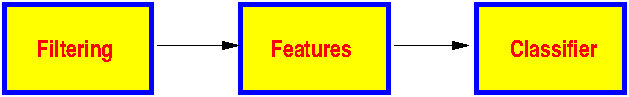
\includegraphics [height=20mm] {images/bildchen}
\caption {Aufbau eines Mustererkennungssystems}
\label{fig:AufbauMustererkennungssystem}
\end{figure}

Auch andere Grafikformate werden unterstützt. Verwenden Sie den Assistenten in TeXstudio, um komfortabel Grafiken einzufügen. Siehe dazu \autoref{fig:GrafikEinfuegen}. Die Grafiken finden sich nicht notwendigerweise direkt am Einfüge-Ort. Das Textsatzsystem richtet es so ein, dass es gut aussieht.

\begin{figure}
\centering
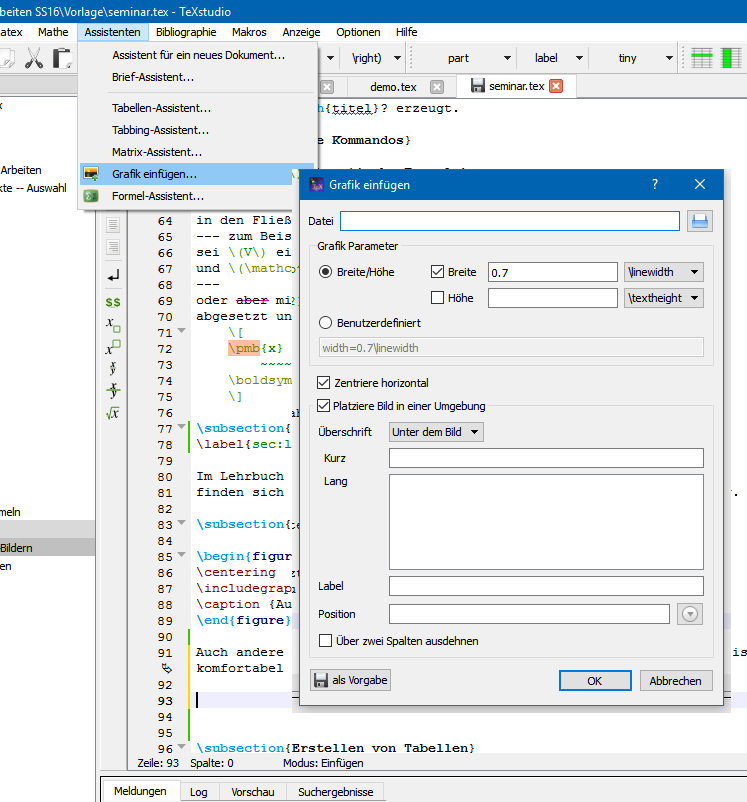
\includegraphics[width=0.7\linewidth]{images/GrafikEinfuegen}
\caption{Verwendung des Assistenten, um eine Grafik einzufügen.}
\label{fig:GrafikEinfuegen}
\end{figure}

\blindtext

\blindtext

\blindtext
\blindtext

\subsection{Querverweise}\label{sec:querverweise}
Verwenden Sie unter TeXstudio die rechte Maustaste in der Strukturübersicht, um für einen Abschnitt ein Label zu erzeugen, auf das Sie Bezug nehmen können (siehe \autoref{fig:LabelErzeugen}).

\begin{figure}
\centering
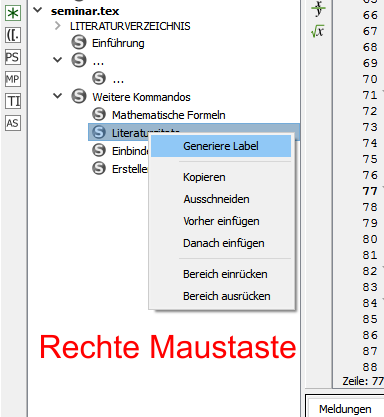
\includegraphics[width=0.4\linewidth]{images/LabelErzeugen}
\caption{Automatische Erzeugung eines Labels für Querverweise}
\label{fig:LabelErzeugen}
\end{figure}

Es wird ein Eintrag \verb|\label{key}| erzeugt, auf den man beispielsweise mit
\verb|\autoref{key}| verweisen kann. Verwendet man \verb|\autoref|, wird der Typ des Objekts
(z.\,B. Abbildung, Tabelle, etc.) mit ausgegeben. Verwendet man nur \verb|\ref|,
so wird nur die Nummerierung des Objekts ausgegeben.

\subsection{Erstellen von Tabellen}

Das Volk hat gesprochen. Siehe \autoref{tab:tabular}. Auch hier kommt ein float zum Einsatz, jedoch mit dem Positionierungs-Hinweis \verb|[h]|. Jedes float sollte mit einem Label versehen werden, und es sollte im Text darauf verwiesen werden, da sich die Position ändern kann.

\begin{table}[h]
\centering
\begin{tabular} {|llc||r|}
	\hline
	Name & Rang & Fraktion & Stimmenanteil \\
	\hline
	Mobutu & General & CDU & 57\% \\
	Tsvangirai & Oberst & CSU & 63\% \\
	\hline
\end{tabular}
\caption {Bundestagswahl in Simbabwe}
\label{tab:tabular}
\end{table}

\autoref{tab:booktab} verwendet keine vertikalen Linien und entspricht dem üblicherweise in Büchern verwenden Stil. Derartige Tabellen sind deutlich ansehnlicher.

\begin{table}[h]
\centering
\begin{tabular} {llcr}
	\toprule
	Name & Rang & Fraktion & Stimmenanteil \\
	\midrule
	Mobutu & General & CDU & 57\% \\
	Tsvangirai & Oberst & CSU & 63\% \\
	\bottomrule
\end{tabular}
\caption {Bundestagswahl in Simbabwe}
\label{tab:booktab}
\end{table}

\subsection{Listen und Aufzählungen}

Listen und Aufzählungen werden in einer Umgebung angelegt (umschlossen von \verb|begin| und \verb|end|.). \verb|\begin{itemize}| leitet eine Liste ein und \verb|\begin{enumerate}| eine Aufzählung. Die Einträge werden jeweils mit \verb|\item| begonnen. Folgend zwei Beispiele.

Itemize:
\begin{itemize}
\item Test
\item Test
\item Test
\end{itemize}

Enumerate:
\begin{enumerate}
\item Test
\item Test
\item Test
\end{enumerate}

%
%	Theorieteil
%

\pagebreak
\section{Management of Container Platforms in the Enterprise}

\onehalfspacing

\subsection{Key requirements in Enterprise IT}

A crucial component of security when running container in production, according to NIST, is separation\footnote{Vgl. \textit{Souppaya, M. (2017)}: Application Container Security Guide \cite{sp800-190}}.

Many enterprises will end up with more than one Kubernetes cluster, sometimes with many more.

\begin{figure}[h]
\centering
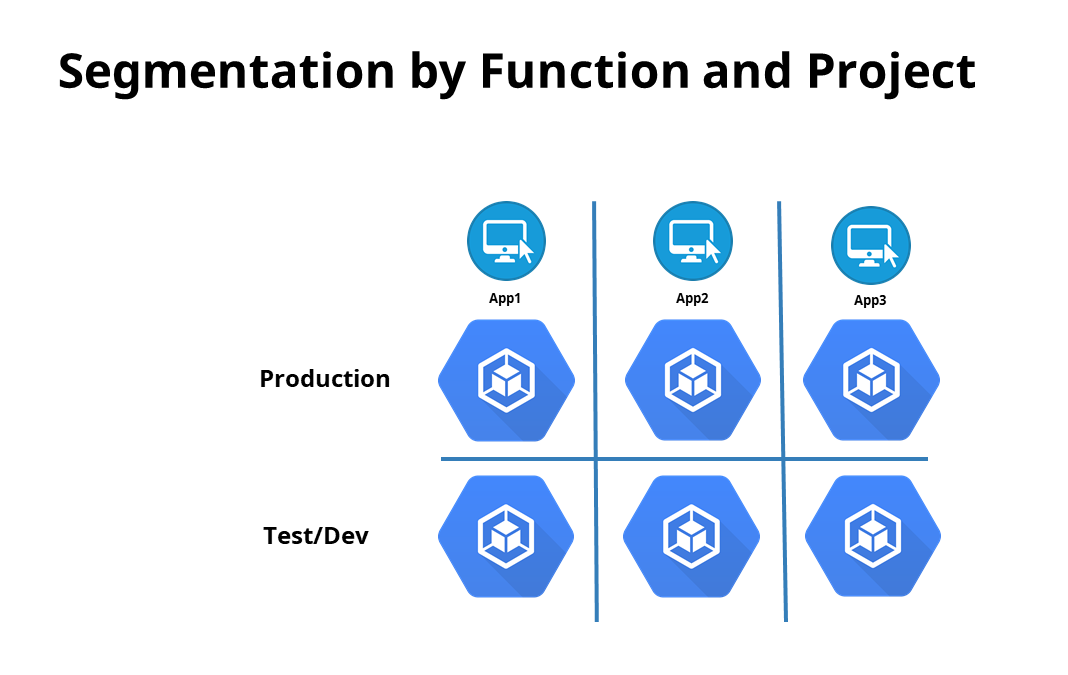
\includegraphics[width=\linewidth]{images/separation}
\caption {Cluster Separation}
\label{fig:clusterSeparation}
\end{figure}

\subsection{Issues when running multiple Kubernetes clusters}

If you run more than one cluster, you'll need to synchronise a lot of tasks across all these clusters

\begin{itemize}
\item User Authentication
\item Roles and Responsibilities
\item Security Policies
    \begin{itemize}
    \item Pod Security Policies
    \item Network Security Policies
    \end{itemize}
\item Applications
\item Versions
    \begin{itemize}
    \item Cluster 
    \item Applications
    \end{itemize}
\end{itemize}

to name a few

Also, you might want to connect your software development pipeline to the various Kubernetes clusters or install a service mesh

\subsection{Possible solutions}

Kubernetes provides a multi-cluster controller, but it's still in its infancy.

Google have Anthos\footnote{Vgl. \textit{Google (2019)}: Anthos - Bringing the cloud to you \cite{googleAnthos}} to address this issue, Microsoft have Azure Arc\footnote{Vgl. \textit{Microsoft (2019)}: Bring Azure services and management to any infrastructure \cite{azureArc}} in Preview

An Open-Source solution for this problem is Rancher\footnote{Vgl. \textit{Rancher Labs (2019)}: Run Kubernetes Everywhere \cite{rancher}}, by Rancher Labs.


%
%	Praxisbezug
%

\pagebreak
\section{Using Rancher as an Enterprise Container Management Platform}

\onehalfspacing

\blindtext


%
%	Fazit
%

\pagebreak
\section{Summary and recommendations}

\onehalfspacing

In summary, we have seen that Rancher currently provides an excellent tool to manage multiple Kubernetes clusters in Enterprise IT.

There are other options though: Google are developing Anthos, AWS have Outpost and Microsoft have Azure Arc (in preview) - all these tools are aimed at extending the management capabilities of the respective cloud provider to other public cloud platforms and in-house data centers.

For the time being, Rancher is the only open-source, provider independent solution and the recommended choice.

There are new changes on the horizon that threaten infrastructure itself: With the advent of functions and Event Driven Architecture new patterns emerge in cloud native application design that have the potential to render virtualization and containerization obsolete. Main contenders in this space are AWS Lambda, Google Cloud Run, Google Cloud Functions, and Microsoft Functions.

Also, AWS and CloudFlare are developing new container run-time environments and the introduction of micro-VMs; the biggest announcement at the end of 2019 was the introduction of Kubernetes on Fargate by AWS\footnote{Vgl. \textit{AWS (2019)}: Run Serverless Kubernetes Pods Using Amazon EKS \cite{eksFargate}}.

There are a lot of developments coming in 2020 with uncertain outcomes, however, what we can say for sure is that software will eat the world (of infrastructure).


% Literaturverzeichnis
\cleardoublepage
\raggedright
\bibliographystyle{IEEEtranS}	% ieeetran verwenden, damit auch URLs angezeigt werden
\bibliography{seminar-lit}
\end{document}
